\documentclass[10pt,a4paper]{article}

\usepackage[a4paper,margin=1.6cm]{geometry}
\usepackage[T1]{fontenc}
\usepackage{lmodern}
\usepackage{microtype}
\usepackage{amsmath}
\usepackage{amssymb}
\usepackage{graphicx}
\usepackage{booktabs}
\usepackage{tabularx}
\usepackage{enumitem}
\usepackage{caption}
\usepackage{titlesec}
\usepackage[hidelinks]{hyperref}

% Same compact layout as the two previous reports.
\setlist{nosep, leftmargin=*}
\titleformat*{\section}{\large\bfseries}
\titleformat*{\subsection}{\normalsize\bfseries}
\titlespacing*{\section}{0pt}{1.1ex}{0.5ex}
\titlespacing*{\subsection}{0pt}{0.8ex}{0.3ex}
\captionsetup{font=small, labelfont=bf, skip=3pt}
\setlength{\parindent}{0pt}
\setlength{\parskip}{0.5ex}
\newcommand{\code}[1]{\texttt{#1}}

\begin{document}

\begin{center}
  {\Large\bfseries Learning Agent Code Report}\\[3pt]
  Time-Aware Reinforcement Learning for Ball Catching under Visual Delay\\[2pt]
  ME5418 Group 30
\end{center}

%==========================================================================================
\section{Code Explanation}

The learning agent connects the two previous milestones: it plays a network from \code{networks/}
in the Gym environment of \code{ball\_catch/} and trains it with PPO. The new code is a package
\code{agent/}, a training script \code{train.py}, a parallel rollout collector added to
\code{networks/ppo.py}, an input-standardisation layer in the networks and a \code{-{}-model} option
for \code{demo.py}. Tests cover training, recurrent memory, saving/loading and safe output handling.
The three policies are a memoryless MLP (9 inputs), a 64-unit GRU (9 inputs), and the same GRU with
capture interval and observation age added (11 inputs). All output a Gaussian action and a value estimate.

\subsection{Organisation}

\begin{tabularx}{\textwidth}{@{}lX@{}}
  \toprule
  File & What it does \\
  \midrule
  \code{agent/ppo\_agent.py}  & \code{TrainConfig} (every hyperparameter, saved with the model) and \code{PPOAgent}:
                                 \code{update}, \code{train}, \code{evaluate}, \code{save}; \code{load\_policy}. \\
  \code{agent/controller.py} & \code{NetworkController}: a trained network behind the interface of the hand-written
                                 controllers, so that it is evaluated and displayed by the same code. \\
  \code{networks/ppo.py}     & New \code{RolloutCollector} (several environments, one batched network call per step)
                                 and \code{Rollout.select} (a minibatch of environments). \\
  \code{train.py}            & Command line: training log (CSV), learning curve, checkpoint, final comparison. \\
  \code{demo.py -{}-model}   & Watches or evaluates a trained network in the live window, a GIF, or statistics only. \\
  \bottomrule
\end{tabularx}

\subsection{One PPO update}

\textbf{1. Collect.} 16 environments run in lockstep for 128 control steps (2{,}048 steps, about 38
throws). At each step one network call returns, for all environments, the sampled actions, their
log-probabilities, the values and the new GRU memory. A finished throw is reset at once and marked
\code{episode\_start}, where the network clears its memory. Throws and memory carry over to the next rollout.

\textbf{2. Advantages.} GAE with $\gamma$ and $\lambda$ from the table below; there is no bootstrapping
across the end of a throw, and the critic's value after the last step bootstraps the unfinished ones.

\textbf{3. Learn.} 10 epochs over the rollout, each split into 4 minibatches of 4 environments.
A minibatch keeps every sequence whole, and the GRU is re-run from the memory it had at the start of the
rollout, so before the first gradient step the re-computed log-probabilities equal the stored ones
(a unit test checks this). Each minibatch takes one Adam step on the clipped PPO policy loss plus
$0.5$ times the value mean-squared error, with gradient norm clipped to 0.5 and a linear learning-rate decay.

\textbf{4. Inputs.} A new first layer, \code{ObservationNorm}, standardises each input with the running mean
and variance of all observations so far. It is updated only after the learning phase, so a rollout is
collected and re-evaluated with the same statistics, and it is saved with the weights.

{\small
\begin{tabularx}{\textwidth}{@{}lX|lX@{}}
  \toprule
  Rollout  & 16 environments $\times$ 128 steps            & Discount $\gamma$, GAE $\lambda$ & 0.995, 0.95 \\
  Learning & 10 epochs $\times$ 4 minibatches of 512 steps & Clip, value / entropy weight     & 0.2, 0.5 / 0 \\
  Adam     & lr $3\times10^{-4}$ decayed linearly to 0, $\epsilon = 10^{-5}$ & Gradient norm & clipped to 0.5 \\
  Budget   & 3\,M steps per run; 3 seeds per network      & Inputs                           & running standardisation \\
  \bottomrule
\end{tabularx}
}

\subsection{Evaluation across three training seeds}

Each network uses training seeds 0, 1 and 2, with identical hyperparameters and 3\,M steps per run
(1{,}465 updates; 3{,}000{,}320 actual steps). We retained the original seed-0 checkpoints and trained
seeds 1 and 2 afresh. Training stream $i$ starts from seed $16s+i$ for run seed $s$.
\code{PPOAgent.evaluate} uses mean actions on the same 1{,}000 throws (seeds 100{,}000--100{,}999),
so every policy faces identical throws, sensor noise and delays. We evaluate the final checkpoint,
not the best intermediate score.

The temporal network catches $28.0\pm3.2\%$, the recurrent network $22.6\pm3.0\%$, and the single-frame
network $13.4\pm1.2\%$ (mean $\pm$ sample standard deviation across training seeds).
Temporal exceeds recurrent in all three runs by 4.9, 5.8 and 5.3 percentage points, averaging 5.3 points.
This is preliminary evidence on this benchmark, not a general claim: only three training seeds were
tested, and the evaluation set was also used for monitoring and tuning. The privileged oracle still
catches 97.4\%, leaving considerable room to improve interception accuracy.

\begin{figure}[h]
  \centering
  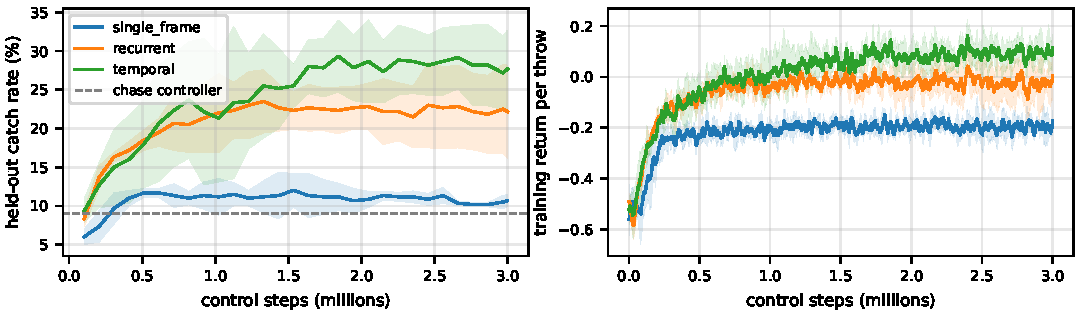
\includegraphics[width=\textwidth]{figures/learning_curves_multiseed.pdf}
  \caption{Jitter delay; seeds 0, 1, 2. Lines: means; bands: $\pm1$ sample SD across training seeds.
    Left: mean-action catch rate on 200 held-out throws every 50 updates, plus the final update;
    the chase reference uses the same 200 throws.
    Right: exploring-policy return, smoothed over 10 updates per run before averaging.
    Generated by \code{report/summarize\_seeds.py}; final evaluation uses 1{,}000 throws per model.}
  \label{fig:curves}
\end{figure}

\begin{table}[h]
  \centering\small
  \caption{Final checkpoints on the same 1{,}000 held-out throws. Networks: mean $\pm$ sample SD over
    three training seeds; fixed controllers have no training-seed variation.}
  \label{tab:results}
  \begin{tabular}{@{}lrrr@{}}
    \toprule
    Controller & Caught (\%) & Mean return & Mean miss distance (m) \\
    \midrule
    Stationary                       & $5.3$          & $-0.41$          & $0.70$ \\
    Chase (hand-written)             & $10.5$         & $-0.27$          & $0.55$ \\
    \code{single\_frame} network     & $13.4\pm1.2$  & $-0.18\pm0.03$  & $0.51\pm0.02$ \\
    \code{recurrent} network         & $22.6\pm3.0$  & $0.00\pm0.08$   & $0.43\pm0.05$ \\
    \code{temporal} network          & $28.0\pm3.2$  & $+0.11\pm0.05$  & $0.37\pm0.02$ \\
    Oracle (privileged, delayed start) & $97.4$        & $+1.37$          & $0.03$ \\
    \bottomrule
  \end{tabular}
\end{table}

\noindent\begin{minipage}{\textwidth}
\textbf{How to run.}
{\small
\begin{verbatim}
python train.py --out runs/new_temporal   # temporal network; preserves the supplied checkpoints
python run_seeds.py --seeds 1 2           # all three variants, two jobs at a time
python demo.py --model runs/temporal_jitter_seed0/model.pt   # watch the trained network
python -m unittest                       # environment, networks, agent and script tests
\end{verbatim}
}
\end{minipage}

%==========================================================================================
\section{Existing Codes and Libraries}

\begin{itemize}
  \item \textbf{PyTorch 2.5.1}: Adam, \code{clip\_grad\_norm\_}, saving and loading of weights;
        \textbf{Matplotlib 3.7.5} for the learning curves.
  \item \textbf{Our environment and networks} (previous milestones), used through \code{BallCatchEnv},
        \code{make\_policy}, \code{act} and \code{evaluate}, and \code{ball\_catch.evaluation}.
        \textbf{Gym 0.26.2} supplies the environment API; \textbf{NumPy 1.23.5} the simulation and random
        numbers; \textbf{Pillow 10.4.0} GIF export. No external simulator is required.
        Python 3.9.25 and dependency versions are pinned in \code{environment.yml}; setup is in README.
  \item \textbf{Method references}: PPO (Schulman et al., 2017) and GAE (Schulman et al., 2016). The
        update follows the CleanRL single-file implementations: Adam with $\epsilon = 10^{-5}$,
        gradient clipping, linear learning-rate decay and the KL estimate $\mathbb{E}[(r-1)-\log r]$
        from \code{ppo\_continuous\_action.py}; minibatches of whole environment sequences with their
        initial memory from \code{ppo\_atari\_lstm.py}. We wrote our own code from these descriptions.
\end{itemize}

%==========================================================================================
\section{Reflections and Lessons Learned}

\textbf{Design choices.}
\begin{itemize}
  \item \textbf{Minibatches of whole sequences.} A throw lasts at most 72 steps and a rollout 128, so each
        minibatch re-runs a complete 128-step sequence from its stored initial memory. Gradients are
        truncated at rollout boundaries; no additional chunking or burn-in is used.
  \item \textbf{Throws continue across rollouts.} Restarting every environment at each rollout would
        over-represent the beginning of throws, and the last throw of every rollout would be cut short.
  \item \textbf{Independent runs.} One CPU thread per job; \code{run\_seeds.py} queues two jobs at a time.
        Separate output folders and overwrite checks preserve the models used in the report.
\end{itemize}

\textbf{Lessons from repetition.} The original temporal result was 28.6\%; additional seeds reached
30.8\% and 24.5\%. A single run therefore hides meaningful variation. We fixed the training budget
and hyperparameters before these repeats, and report all final checkpoints instead of selecting
the best seed. The summary script checks that checkpoints, logs and evaluation protocols agree;
per-run CSV and summary JSON accompany the figure. Sample SD is not a confidence interval.

\textbf{Next steps.} Reserve an untouched evaluation set; test fixed delays of 0--0.2\,s and unseen burst
delays; add the predictive estimator with a PD controller; and check action saturation, using tanh
squashing if mean actions frequently exceed $\pm1$. More training seeds are needed for broader conclusions.

\textbf{AI tool declaration.} We used Claude and GPT, through the AI assistant, to help design, write and
test the agent code, and to draft and optimise this report. The requirements for the project were proposed by us after
discussion. We are responsible for the content and quality of the submitted work.

\end{document}
